\documentclass[../main.tex]{subfiles}

\begin{document}
	\section{Architektur}
	\todo[inline]{Erste Basisarchitektur definieren}
	Wegen der Vielfältigkeit und möglicher Komplexität der eingesetzten Technologien, ist eine klare Architektur der Software ein wichtiger Faktor. Dennoch sollte diese stets erweiterbar sein, da das Produkt stetigen weiterentwickelt wird und eine verfrühte Festsetzung, an einem späteren Zeitpunkt, zu negativen Auswirkungen führen kann.\\
	Für die Dokumentation wir auf die bestehenden Werkzeuge und Möglichkeiten von Unity und C\# zurückgegriffen.\\
	Als Sprache im Code wird ausschliesslich Englisch eingesetzt.\\
	In den folgenden Abschnitten wird auf die bereits getroffenen Entscheide, für die Realisierung des \gls{mvp}, eingegangen.
	
	\subsection{Ansatz}
	Unity, als eingesetzte Technologie, zielt auf ein sehr breites Publikum ab. Dabei wird nicht nur einen einzigen Lösungsansatz verfolgt, stattdessen lässt es mehrere Ansätze zu, welche auch gemischt werden können. Um die Struktur im gesamten Projekt konstant halten zu können, wird im allgemeinen der Klassen-orientierter Ansatz verfolgt. Dabei wird der Augenmerk auf die Programmierlogik gelegt anstelle der Komponenten oder Spielobjekte.\\
	Beim Klassen-orientierten Ansatz wird versucht, die Logik des Spiels von der Darstellung dieses so weit wie möglich zu trennen. Durch solch eine Trennung kann Logik und Visualisierung Parallel designed und entwickelt werden. Ausserdem, kann die Logik des Spiels separate getestet werden.
	
	
	\subsection{Koordinatensystem}
	\label{coordinatessystem}
	Obwohl die Logik des Spiels sich auf zwei Dimensionen beschränkt, eignet sich das drei dimensionale kartesische Koordinaten System besser. Der Grund dafür ist die hexagonale Art des Spiels wobei sich jede der Achsen des Hexagons zu einer der Achsen des Koordinaten Systems zuordnen lässt.\\
	Der Einsatz des kubischen Koordinaten Systems bringt ausserdem einige Vorteile mit sich. Zum einen ist eine eindeutige Einteilung des Spielfelds möglich. Zum anderen ist der Einsatz von existierenden Algorithmen möglich, die für 3 Dimensionen ausgelegt sind, wie zum Beispiel:
	\begin{itemize}
		\item Pathfinder Algorithmen
		\item Lineare Suchalgorithmen
		\item Lösungsalgorithmen
		\item Baum Traversierung
	\end{itemize}
		
	\begin{figure}[H]
		\centering
		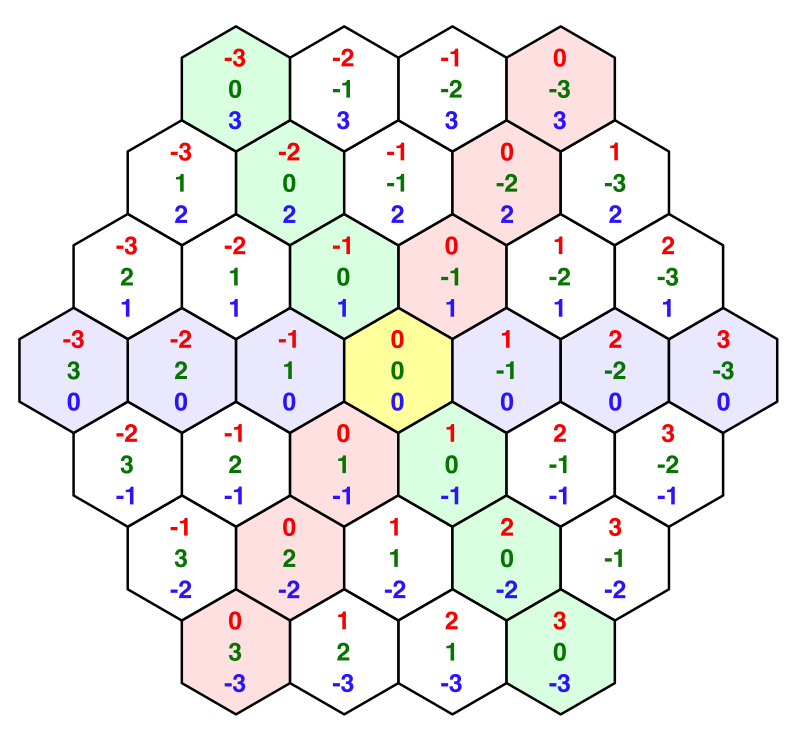
\includegraphics[width=0.5\textwidth]{coordinate-system}
		\caption{drei Dimensionales Koordinaten System}
	\end{figure}
	
	\subsection{Einheitensystem}
	Die Schlichtheit des Spiels erfordert grundlegend nur ein Einheitensystem; benötigt für die Visualisierung des Spielfeldes. Hierbei kommt ein anderer Vorteil des kubischen Koordinatensystems (\ref{coordinatessystem}) zum Vorschein. Die Position eines jeden Plättchens erfolgt entlang der jeweiligen Achsen multipliziert mit den der Position auf dieser. Somit ist keine komplexe Kalkulation erforderlich, stattdessen eine triviale dreifache Multiplikation. Die Einheit dabei ist die Distanz zwischen den Zentren der einzelnen Plättchen, was gleichzeitig der "Durchmesser" des Plättchens ist. Dabei spielt die Grösse der Plättchen keine Rolle, solange diese stets einheitlich gross sind.\\
	Die Einheit der Distanz ergibt sich somit aus dem Durchmesser des Plättchens und ist als Einheit \textbf{1} zu verstehen.
	
	Weitere Einheiten sind im gegenwärtigen Stand des Spiels nicht erforderlich, können jedoch jederzeit mit aufgenommen werden. 
	
	\subsection{Beschränkungssystem}
	Das Beschränkungssystem ist der Kern der Logik des Spiels. Dieses System ist dafür zuständig die logische Korrektheit des Spiels zu gewährleisten. Dabei werden Beschränkungen definiert, die \heavy{unabhängig} vom eigentlichen Quellcode des Spiels getrennt sind. Das System verarbeitet diese Definition und setzt die Logik in das Spiel um. Solch eine Trennung zwischen Spielimplementierung und Logik hat den Vorteil diese eigenständig verfeinern zu können, jedoch auf kosten einer erhöhten Komplexität.\\
	Dabei soll die Definition so variable wie möglich gehalten werden ohne die Komplexität des Systems zu sprängen. Die möglichen Beschränkungen im System sind eingegrenzt auf die Faktoren: Position, Farbe, Punkte und die Interaktion zwischen diesen. Mögliche Beispiele aber nicht nur ausschliessliche Beschränkungen wären zum Beispiel:
	\begin{itemize}
		\item Distanz des nächst möglichen Plättchen
		\item Zugarten:
		\begin{itemize}
			\item Achsen gebunden
			\item Springer beim Schach
		\end{itemize}
		\item Restriktionen der Farben zu einander
		\item Auswirkung der Punkte auf andere Faktoren wie die Distanz
	\end{itemize}
	
	Zum gegenwärtigen Zeitpunkt ist der Ausbau dieses Systems noch nicht endgültig definiert. Als Grundlage dient in erster Linie eine tabellarische Darstellung der Beschränkungsbeschreibungen kann aber, zu einem späteren Zeitpunkt, durch eine einfache formale Sprache abgelöst werden.
	
	
\end{document}